\section{Untersuchung der Fertigungsdurchführung}\label{sec:untersuchung}

Aus Kapitel \ref{ch:einleitung} ist bekannt, dass in der vorliegenden Bachelorarbeit speziell im Geschäftsprozess der Fertigungsdurchführung in SAP S/4HANA Cloud nach Aktivitäten gesucht werden soll, die Potenziale für den Einsatz von Ereignisverarbeitung und Automatisierung bieten. 
Nachdem in Kapitel \ref{ch:Grundlagen} die Automatisierung von Geschäftsprozessen mittels Ereignisverarbeitung allgemein betrachtet wurden, wird die Fertigungsdurchführung als exemplarischer Untersuchungsgegenstand dieser Bachelorarbeit nun im Kontext der Geschäftsprozessanalyse betrachtet. 

\subsection{Methodisches Vorgehen zum Experteninterview}
Mithilfe von Experteninterviews werden möglichst alle in der Praxis als Standard geltenden Aufgaben in der Fertigungsdurchführung empirisch erhoben.
\cite{Kaiser.2014}
Aus den korrespondierenden Informationen werden Kriterien für die zu findenden Maßnahmen zur Automatisierung aufgestellt. 
Da Experteninterviews in dieser Bachelorarbeit keineswegs die einzige Methode darstellen, sondern lediglich zusätzliches Wissen liefern, ist eine ausgewählte Stichprobe der für das Thema relevanten Perspektiven im vorliegenden Fall ausreichend.

Das Wissen darüber, welche Aufgaben in der Fertigungsdurchführung allgemein sowie mit SAP S/4HANA Cloud als unabkömmlich gelten und welche Merkmale und Defizite diese aufweisen, ist extrem unternehmensspezifisch und kann daher ausschließlich durch ausreichend Erfahrung generalisiert dargestellt werden. 
Laut \citeauthor{Mieg.2005} braucht es in etwas 10 Jahre Erfahrung in einem Themengebiet, um als Experte zu gelten.
\cite{Mieg.2005} Den Protokollen der Interviews im Anhang \ref{ah:protokolle} ist zu entnehmend das dieses Kriterium als übererfüllt betrachtet werden kann.
Zugleich ist es das erforderte Wissen in einschlägiger Literatur nicht auffindbar.
Die ausgewählten Experten sollten daher Repräsentanten verschiedener Perspektiven auf den Geschäftsprozess darstellen, sodass die Ergebnisse möglichst generalisierbar sind. 
Bei der Auswahl der Experteninterviews wurden folgende Perspektiven beachtet:

\begin{itemize}
    \item 
    \textbf{Branchenexperte}: Dieser vertritt die Rolle des externen Stakeholders. Er hat ein eigenes Interesse am Ablauf des Geschäftsprozesses und war selbst schon in der Planung und Durchführung des Geschäftsprozesses beteiligt. 
    \item
    \textbf{Prozessexperte}: Als Prozessexperte wird im Kontext dieser Bachelorarbeit eine Person verstanden, zu deren Kerngebieten der ausgewählte Geschäftsprozess gezählt wird. Er arbeitet zusammen mit Kunden im SAP-Umfeld an der Einführung und Optimierung des Geschäftsprozesses
    \item
    \textbf{Technologieexperte}:  Ein Technologieexperte beschäftigt sich eingehend mit den technologischen Hilfsmitteln des Geschäftsprozesses, sowie mit deren Verwendung und Implementierung in SAP S/4HANA Cloud.
\end{itemize}

Bei empirischen Untersuchungen ist des Weitere  zwischen qualitativen und quantitativen Untersuchungen zu unterscheiden. Während qualitative Verfahren die Gemeinsamkeiten von mehreren Gegebenheiten untersuchen indem existierende Unterschiede überwunden werden, erfasst die quantitative Sozialforschung Unterschiede auf Vergleichsbasis von Gemeinsamkeiten. Für die empirische Untersuchung der Fertigungsdurchführung auf Möglichkeiten zur Integration von Betriebswirtschaft und Informationstechnologie wird die qualitative Methode gewählt. 

Damit alle Informationen ordnungsgemäß und nachvollziehbar erhoben werden und alle Erkenntnisse wissenschaftlich fundiert sind, werden die Experteninterviews nach dem untenstehenden Vorgehen strukturiert durchgeführt.

\begin{enumerate}
    \item 
    \textbf{Identifikation eines Experten}: Nur eine Person, die ausreichend Erfahrung im Bereich \ac{PPS} und auf dem Gebiet der Fertigungsdurchführung gesammelt hat, ist in der Lage, Merkmale und Defizite in den Aktivitäten dieses Geschäftsprozesses zu erkennen und zu benennen. Es werden also Personen benötigt, die spezifisches Rollenwissen besitzen und somit als kompetent und erfahren angesehen werden. \cite{Mieg.2005}
    \item
    \textbf{Entwicklung eines Fragebogens}: Die Qualität und der Nutzen eines Experteninterviews hängen stark vom Fragebogen ab. Die Fragen für diese Arbeit werden daher mit großer Sorgfalt gesammelt, woraufhin sie vom Autor dieser Bachelorarbeit genau geprüft und sortiert werden. Die Fragen sind so formuliert, dass sie bewusst sehr präzise Antworten hervorrufen.
    \item
    \textbf{Formung und Vorstrukturierung des Interviewablaufs}: Zu Beginn der Experteninterviews werden formale Informationen akquiriert und Wünsche der Experten entgegengenommen. 
    Für die Experteninterviews wird jeweils eine Zeitspanne von 30 bis 60 Minuten angesetzt. Als Interviewer fungiert der Autor dieser Bachelorarbeit.
    \item
    \textbf{Gestaltung der an dem Interview beteiligten Rollen}: Zwischen den Experten und dem Interviewer liegt augrund der Erfahrung und der Vorkenntnisse eine wissensbezogene Disparität zugunsten der Experten vor. Um also möglichst viele Informationen von der Expertin zu erhalten, gewährt der Interviewer den Experten einen maßgeblich größeren Teil der gesamten Redezeit.
    \item
   \textbf{ Durchführung des Experteninterviews}: Die Experteninterviews wird werden online via Skype durchgeführt. Nachdem eine Frage gestellt wird, erhalten die Experten eine variable Antwortzeit. Gemäß des Fragenkatalogs geben Experten die gewünschten Informationen an den Interviewer weiter.
    \item
    \textbf{Nachbereitung und Kernaussagen des Experteninterviews}: Die Notizen aus dem Experteninterview werden inhaltlich, sprachlich und strukturell aufbereitet. Die Kernaussagen werden summarisch zusammengefasst. \footnote{Dies wurde mit dem wissenschaftlichen Betreuer dieser Bachelorarbeit entsprechend abgestimmt.} Die summarischen Kernaussagen sind im Anhang \ref{ah:protokolle} abgelegt.
\end{enumerate}

\subsection{Interpretation der Ergebnisse aus den Experteninterviews}
Zur Sicherung der Ergebnisse, welche mithilfe der leitfadengestützten Experteninterviews erzielt wurden, wurden die Aussagen des Experten in verschiedenen Formen festgehalten. Zusätzlich dazu liegt das Interview als Audioaufzeichnung vor. 

Basierend auf den relevanten Kernaussagen der befragten Experten , die im Anhang \ref{ah:protokolle} aufgeführt und mit Bezeichnern versehen sind, werden nun typische Merkmale und Defizite der Fertigungsdurchführung in der diskreten Fertigung identifiziert und dargestellt. 
Mit Hilfe der vergebenen Bezeichnern wird im Folgenden auf die einzelenen Kernaussagen Bezug genommen.
Damit dienen diese Kernaussagen der Untersuchung der Fertigungsdurchführung in der praktischen Wirklichkeit eines Industriebetriebs.
Da diese Kernaussagen aus den Ergebnissen der Experteninterviews abgeleitet sind, sind sie schwierig operationalisierbar und nicht widerspruchsfrei.  
Sie lediglich dazu, die Erkenntnisse der Experteninterviews zu sammeln und zu verdichten.


\subsection{Merkmale und Defizite der Fertigungsdurchführung}
Die Freigabe eines Fertigungsauftrags ist sowohl in der Literatur (siehe Abschnitt \ref{sec:untersuchung}) wie auch in den Kernaussagen der befragten Experten als auslösendes Ereignis der Fertigungsdurchführung anzusehen. ($\rightarrow$ \textbf{KA-B-1} und \textbf{KA-P-1})  
In diesem Zusammenhang zeichnet sich die Freigabe des Fertigungsauftrags mit der Eigenschaft, nur geringfügig flexibel und schnell zu sein, aus. Diese Erkenntnis ist darauf zurückzuführen, dass die Fertigungsdurchführung auf der operativen Ebene der Produktion in der Praxis auch heute noch zum großen Teil auf Papier basiert. Dies hat zur Folge, dass vermehrt Latenzzeiten in der Produktion, aufgrund von Abholungen und Abgaben der Fertigungsdokumente, auftreten. 

Eine weitere Übereinstimmung von Literatur und Praxis stellt die Rückmeldung zur Erfassung der Betriebsdaten in der Fertigungsdurchführung dar. Als notwendige Informationen die zwangsläufig in einer Rückmeldung erfasst werden müssen werden die \textit{Auftragsnummer, Vorgangsnummer, Gut-, Ausschuss- und Nacharbeitsmenge sowie die Durchlaufszeiten} angesehen.
($\rightarrow$ \textbf{KA-B-6}, \textbf{KA-P-6} und \textbf{KA-T-3})  

In der Praxis werden der Rückmeldung von Fertigungsaufträgen jedoch eine geringe Transparenz
($\rightarrow$ \textbf{KA-B-2} und \textbf{KA-P-2}), einen hohen Erfassungsaufwand
($\rightarrow$ \textbf{KA-B-3},\textbf{KA-P-3}) sowie eine mangelhafte Datenqualität
($\rightarrow$ \textbf{KA-B-4}, \textbf{KA-P-4} und \textbf{KA-T-1}) attestiert. 
Dies lässt sich auf die, in der Regel manuelle, Erfassung von Informationen in Papierform inklusive einer nachträglichen Übertragung in SAP S/4HANA Cloud zurückführen. Der Wechsel des Mediums, der in Abbildung \ref{fig:Typische Prozessschritte der Fertigungsdurchführung} illustriert ist, verursacht eine Doppelerfassung der Betriebsdaten und eine Unterbrechung in der Echtzeitverarbeitung der Informationen. 

\begin{figure}[H]
	\centering 
    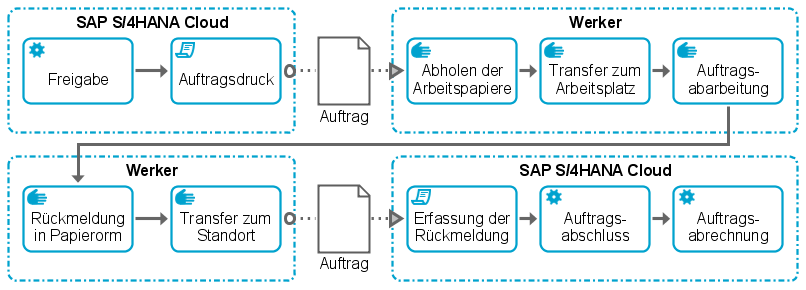
\includegraphics[width=\textwidth]{img/paper.png}	
    \caption[Typische Prozessschritte der Fertigungsdurchführung]
    {Typische Prozessschritte der Fertigungsdurchführung\protect\footnotemark}
    \label{fig:Typische Prozessschritte der Fertigungsdurchführung}
\end{figure}
\footnotetext{Eigene Darstellung}
\footnotetext{Die Abbildung dient lediglich der Visualisierung und ist nicht \ac{BPMN} 2.0 konform.}

Zeitnahe Informationen sind durch die Verwendung von Papier in der Fertigungsdurchführung kaum möglich und führen so zu einer erheblich schlechteren Transparenz im Geschäftsprozess, was sich maßgeblich auf die Reaktionsfähigkeit der Produktionssteuerung auswirkt. Die Papiere müssen wie auch bei der Freigabe eines Fertigungsauftrags transportiert werden, was wiederum zu Latenzzeiten führt und sich somit in der Durchlaufszeit der Fertigungsaufträge niederschlägt.